% This is samplepaper.tex, a sample chapter demonstrating the
% LLNCS macro package for Springer Computer Science proceedings;
% Version 2.20 of 2017/10/04
%
\documentclass[runningheads]{llncs}

\usepackage{graphicx}
\usepackage{ae,aecompl}
\usepackage[utf8]{inputenc}
\usepackage[english]{babel}
\usepackage{verbatim}
\usepackage{graphicx}
\usepackage{amsfonts}
\usepackage{amsmath}
\usepackage{amssymb}
\usepackage{stmaryrd}
\usepackage{amstext}
\usepackage{bm} 
\let\proof\relax
\let\endproof\relax
\usepackage{amsthm}
\usepackage{siunitx}
\usepackage{mathrsfs}
\usepackage{wrapfig}
\usepackage{semantic}
\usepackage{algorithm}
\usepackage{algpseudocode}
\usepackage{float}
\usepackage{rotating}
\usepackage[dvipsnames]{xcolor}
\usepackage{paralist}
\usepackage[colorlinks]{hyperref}
\usepackage[capitalise,nameinlink]{cleveref}
\usepackage{url}
\usepackage[nounderscore]{syntax}
\usepackage{environ}
\usepackage{listings}
\usepackage{etoolbox}
\usepackage{subcaption}
\usepackage{alltt}

\AtBeginEnvironment{algorithm}{\linespread{1.05}\selectfont}
\AtBeginEnvironment{grammar}{\small}
\AtBeginEnvironment{grammar}{\linespread{0.6}\selectfont}

% Comments

\newcommand{\simon}[1]{%
  {\scriptsize
      \textbf{\textcolor{red}{Simon: #1}}
  }%
}%

\newcommand{\peter}[1]{%
  {\scriptsize
      \textbf{\textcolor{blue}{Peter: #1}}
  }%
}%

% Paper specific notation

\setlength{\intextsep}{10pt}

\crefname{problem}{problem}{problems}

\newcommand{\inputV}{v}
\newcommand{\consistent}{\ensuremath{\mathit{Consistent}}}
\newcommand{\remaining}{\ensuremath{\mathit{Remaining}}}
\newcommand{\dontcare}{\_}
\newcommand{\defined}{\ensuremath{\mathit{defined}}}
\newcommand{\undefined}{\ensuremath{\mathit{undefined}}}
\newcommand{\properties}{P}
\newcommand{\satisfies}{\vDash}
\newcommand{\simulator}{\mathcal{A}}
\newcommand{\Induced}[2]{\llbracket #1 \rrbracket_{#2}}
\newcommand{\timebase}{\setreal_{\geq 0}}
\newcommand{\stepbase}{\setreal_{> 0}}
\newcommand{\variables}[1]{\mathit{VAR_{#1}}}
\newcommand{\stateset}[1]{S_{#1}}
\newcommand{\runstate}[1]{S^{R}_{#1}}
\newcommand{\state}[1]{s_{#1}}
\newcommand{\inputs}[1]{U_{#1}}
\newcommand{\parameters}[1]{P_{#1}}
\newcommand{\inputvar}[1]{u_{#1}}
\newcommand{\outputs}[1]{Y_{#1}}
\newcommand{\outputvar}[1]{y_{#1}}
\newcommand{\mayReject}{M}
\newcommand{\backtrack}{B}
\newcommand{\values}{\mathcal{V}}
\newcommand{\valuesExchanged}{\mathcal{V_{E}}}
\newcommand{\true}{\mathit{true}}
\newcommand{\false}{\mathit{false}}
\newcommand{\feedthrough}[1]{F_{#1}}
\newcommand{\reactivity}[1]{R_{#1}}
\newcommand{\fset}[1]{\mathtt{set}_{#1}}
\newcommand{\fget}[1]{\mathtt{get}_{#1}}
\newcommand{\fdoStep}[1]{\mathtt{step}_{#1}}
\newcommand{\fpreset}[1]{\mathtt{preSet}_{#1}}
\newcommand{\fpreget}[1]{\mathtt{preGet}_{#1}}
\newcommand{\fpredoStep}[1]{\mathtt{preStep}_{#1}}
\newcommand{\ftime}{\mathtt{ftime}}
\newcommand{\maxStep}[1]{\mathtt{h}_{#1}}
\newcommand{\timestamp}[1]{\varphi(#1)}
\newcommand{\feedsto}[2]{U_{#1}^{#2}}
\newcommand{\CheckCon}{\mathit{CheckConv}}
\newcommand{\stepfound}{\mathit{Step\_found}}
\newcommand{\valuations}{\mathit{V}}
\newcommand{\valuation}{\mathit{v}}


\newcommand{\dom}[1]{\mathit{dom(#1)}}
\newcommand{\algebraic}[1]{\mathit{algebraic_{#1}}}

 

\newcommand{\precondition}{\mathit{Pre}}


\newcommand{\complexity}{Com}
\newcommand{\master}{\mathcal{A}}
\newcommand{\alloutputs}{Y}
\newcommand{\allfeedthroughs}{F}
\newcommand{\allreactivity}{R}
\newcommand{\alldelayed}{D}

\newcommand{\allcontracts}{\mathcal{C}}
\newcommand{\coupling}{L}
\newcommand{\allinputs}{U}
\newcommand{\fmus}{C}
\newcommand{\fmusLoop}{C_{loop}}
\newcommand{\sequence}[1]{\pargroup{#1}}
\newcommand{\functioncall}{f}
\newcommand{\initcall}{I}
\newcommand{\allfunctioncalls}{F}
\newcommand{\fmu}[1]{\texttt{#1}}
\newcommand{\signal}[1]{\texttt{#1}}
\newcommand{\before}[2]{\ensuremath{#1 \twoheadrightarrow #2}}
\newcommand{\ibefore}[2]{\ensuremath{#1 \rightarrow #2}}
\newcommand{\after}[1]{{#1}'}
\newcommand{\aftern}[2]{{#1}^{(#2)}}
\newcommand{\stateafter}[2]{\ensuremath{\state{#1}^{(#2)}}}
\newcommand{\minstep}{\ensuremath{h_{min}}}


\newcommand{\etime}{\ensuremath{E}}

\newcommand{\verifier}{\mathit{Verifier}}

\newcommand{\turnOn}{\mathit{TurnPreconditionsOn()}}
\newcommand{\turnOff}{\mathit{TurnPreconditionsOff()}}

\newtheorem{procedure}{Procedure}{}
\newtheorem{assumption}{Assumption}{}

\newtheorem{experiment}{Experiment}{}

\algrenewcommand\alglinenumber[1]{\scriptsize #1:}% Adapt size of line numbers in algorithm

\algnewcommand\algorithmicforeach{\textbf{for each}}
\algdef{S}[FOR]{ForEach}[1]{\algorithmicforeach\ #1\ \algorithmicdo}
% New definitions
\algnewcommand\algorithmicswitch{\textbf{switch}}
\algnewcommand\algorithmiccase{\textbf{case}}
\algnewcommand\algorithmicassert{\texttt{assert}}
\algnewcommand\Assert[1]{\State \algorithmicassert(#1)}%
% New "environments"
\algdef{SE}[SWITCH]{Switch}{EndSwitch}[1]{\algorithmicswitch\ #1\ \algorithmicdo}{\algorithmicend\ \algorithmicswitch}%
\algdef{SE}[CASE]{Case}{EndCase}[1]{\algorithmiccase\ #1}{\algorithmicend\ \algorithmiccase}%
\algtext*{EndSwitch}%
\algtext*{EndCase}%



% Generic stuff

\newcommand{\footurl}[1]{\footnote{\url{#1}}}

% Math
\newcommand{\brackets}[1]{\ensuremath{ \left[ #1 \right] }}
\newcommand{\tuple}[1]{\ensuremath{ \left\langle #1 \right\rangle }}
\newcommand{\set}[1]{\ensuremath{ \left\{ #1 \right\}}}
\newcommand{\system}[1]{\ensuremath{ \begin{cases} #1 \end{cases}}}
\newcommand{\rightgroup}[1]{\ensuremath{ \left. \begin{matrix} #1 \end{matrix} \right\} } }
\newcommand{\pargroup}[1]{\ensuremath{ \left( #1 \right)}}
\newcommand{\inv}[1]{\ensuremath{\pargroup{ #1 }^{-1}}}
\newcommand{\dert}[1]{\ensuremath{ \dot{#1} }}
\newcommand{\ddert}[1]{\ensuremath{ \ddot{#1} }}
\newcommand{\partialder}[2]{\ensuremath{ \frac{\partial#1}{\partial#2} }}
\newcommand{\setreal}[0]{\ensuremath{\mathbb{R}}}
%\newcommand{\setbool}[0]{\ensuremath{\mathit{Bool}}}
\newcommand{\setnat}[0]{\ensuremath{\mathbb{N}}}
\newcommand{\norm}[1]{\left\lVert#1\right\rVert}
\newcommand{\bnorm}[1]{\big\lVert#1\big\rVert}
\newcommand{\abs}[1]{\left|#1\right\|}
\newcommand{\xs}[2]{\ensuremath{#1^{\left[#2\right]}}}
\newcommand{\infinitynorm}[1]{\left\lVert#1\right\rVert_\infty}


\newcommand{\vectorOne}[1]{\brackets{%
\begin{matrix}
  #1
 \end{matrix}%
}}
\newcommand{\vectorTwo}[2]{\brackets{%
\begin{matrix}
  #1 \\
  #2
 \end{matrix}%
}}
\newcommand{\vectorThree}[3]{\brackets{%
\begin{matrix}
  #1 \\
  #2 \\
  #3
 \end{matrix}%
}}
\newcommand{\vectorFour}[4]{\brackets{%
\begin{matrix}
  #1 \\
  #2 \\
  #3 \\
  #4
 \end{matrix}%
}}
\newcommand{\vectorFive}[5]{\brackets{%
\begin{matrix}
  #1 \\
  #2 \\
  #3 \\
  #4 \\
  #5
 \end{matrix}%
}}
\newcommand{\vectorSix}[6]{\brackets{%
\begin{matrix}
  #1 \\
  #2 \\
  #3 \\
  #4 \\
  #5 \\
  #6
 \end{matrix}%
}}
\newcommand{\vectorSeven}[7]{\brackets{%
\begin{matrix}
  #1 \\
  #2 \\
  #3 \\
  #4 \\
  #5 \\
  #6 \\
  #7
 \end{matrix}%
}}
\newcommand{\vectorEight}[8]{\brackets{%
\begin{matrix}
  #1 \\
  #2 \\
  #3 \\
  #4 \\
  #5 \\
  #6 \\
  #7 \\
  #8
 \end{matrix}%
}}

\newenvironment{aligneq*}%
{
\begin{equation*}
\begin{aligned}
}{
\end{aligned}
\end{equation*}
}

\newenvironment{aligneq}%
{
\begin{equation}
\begin{aligned}
}{
\end{aligned}
\end{equation}
}



%enable \cref{...} and \Cref{...} instead of \ref: Type of reference included in the link
%Nice formats for \cref
\usepackage{iflang}
\IfLanguageName{ngerman}{
  \crefname{table}{Tab.}{Tab.}
  \Crefname{table}{Tabelle}{Tabellen}
  \crefname{figure}{\figurename}{\figurename}
  \Crefname{figure}{Abbildungen}{Abbildungen}
  \crefname{equation}{Gleichung}{Gleichungen}
  \Crefname{equation}{Gleichung}{Gleichungen}
  \crefname{listing}{\lstlistingname}{\lstlistingname}
  \Crefname{listing}{Listing}{Listings}
  \crefname{section}{Abschnitt}{Abschnitte}
  \Crefname{section}{Abschnitt}{Abschnitte}
  \crefname{paragraph}{Abschnitt}{Abschnitte}
  \Crefname{paragraph}{Abschnitt}{Abschnitte}
  \crefname{subparagraph}{Abschnitt}{Abschnitte}
  \Crefname{subparagraph}{Abschnitt}{Abschnitte}
}{
  \crefname{section}{Sect.}{Sect.}
  \Crefname{section}{Section}{Sections}
  \crefname{listing}{\lstlistingname}{\lstlistingname}
  \Crefname{listing}{Listing}{Listings}
}
\crefname{section}{Sect.}{Sect.}
\Crefname{section}{Section}{Sections}
\crefname{listing}{\lstlistingname}{\lstlistingname}
\Crefname{listing}{Listing}{Listings}

\crefname{assumption}{Assumption}{Assumptions}


% update later with official instructions from Springer
\def\orcidID#1{${}^{\smash{\href{https://orcid.org/#1}{\protect\raisebox{-1.25pt}{\protect
\includegraphics{images/orcid_color-eps-converted-to}}}}}$}




% Used for displaying a sample figure. If possible, figure files should
% be included in EPS format.
%
% If you use the hyperref package, please uncomment the following line
% to display URLs in blue roman font according to Springer's eBook style:
% \renewcommand\UrlFont{\color{blue}\rmfamily}

\begin{document}

\title{A Formal Framework for Co-simulation}

\author{Simon Thrane Hansen\inst{1} \orcidID{0000-0002-3796-4319} 
\and Peter Csaba Ölveczky \inst{2} \orcidID{0000-0002-0708-3721}}
%
%\authorrunning{S. Thrane et al.}

\titlerunning{A Formal Framework for Co-simulation}

% First names are abbreviated in the running head.
% If there are more than two authors, 'et al.' is used.
%
\institute{
  DIGIT, Department of Electrical and Computer Engineering, Aarhus University, Aarhus, Denmark, \\
  %\email{\{sth, claudio.gomes, casper.thule\}@ece.au.dk\} 
  \and Department of Informatics, Oslo University, Oslo Norway \\
}

\maketitle              % typeset the header of the contribution

WRLA:\\
\textbf{Deadline: 28th of December}
\\
\textbf{Page limit: 15 (without references)}\\
\textbf{Notification: 8th of February}

\begin{abstract}
Simulation-based analyses of cyber-physical systems are increasingly vital in the era of Industry 4.0. Co-simulation enables the coupling of specialized simulation tools through an orchestration algorithm. 
The orchestrator dictates how each simulation tool should simulate its corresponding subsystem.
Obtaining correct simulation results requires an implementation-aware orchestration algorithm tailored to the specific scenario, without the orchestrator knowing each simulation tool's implementation. 
The orchestrator should stabilize algebraic loops, perform time step negotiation, and adhere to each simulation tool's implementation.
This paper describes an approach and implementation to generate orchestration algorithms that respect all simulation units' implementation contracts by construction using rewriting logic. 
%Furthermore the approach allows one to perform various 
%The approach has been applied to an industrial case study and other complex scenarios. The tool and results are available online.
     
\keywords{Co-Simulation \and Rewriting Logic \and Model-checking \and Cyber-Physical Systems}
\end{abstract}





% Motivation for co-simulation
Cyber-physical systems (CPSs) are omnipresent and part of the critical infrastructure of the modern society.
A CPS is a hybrid system that embodies physical processes controlled by digital devices. Examples include everything from a controller opening and closing a valve to regulate the water level of a tank to autonomous vehicle.
CPSs are becoming increasingly complex and critical~\cite{4519604}, which leads to the desire for techniques to assist in their development.
Traditional modeling and simulation techniques, where a solver algorithm describes a model, are no longer sufficient to cope with the integrated development processes of such systems~\cite{FMI2014}, which consists of heterogenous subsystems typically developed using different tools and techniques~\cite{Monti_2021}. 

% Why and what is co-simulation
%Co-simulation is the study of how to coordinate multiple black-box simulation units (SUs) developed using different tools and formalisms.
Co-simulation solves the shortcomings of the traditional modeling techniques by letting the user couple multiple black-box subsystems (SUs) into a scenario in order to explore the behavior of the combined system as a discrete trace (see, e.g., \cite{Kubler2000,Gomes2018}).

An SU implements a well-defined interface and represents a subsystem by calculating its behavioral trace using a dedicated solver.
An example of such an SU is a Functional Mock-up Unit (FMU) defined by the Functional Mock-up Interface Standard~\cite{FMI2014} (FMI), which inspires the notion of an SU in this paper. 
FMI is widely adopted; supported by many tools~\cite{Tools_FMI} and used commercially.

%How to test and verify an OA - need for correct by construction algorithm
The overarching challenge of co-simulation is ensuring accurate simulation results due to the many potential error sources of such a simulation~\cite{Gomes2018}.
The simulation result depends not only on the SUs but also on the co-simulation algorithm that composes them in a simulation, the later often overlooked~\cite{Gomes2019,Oakes2021,Gomes2018f,Schweizer2015c}.
The co-simulation algorithm must be specifically tailored to the instrumentation of the scenario to ensure an accurate simulation result~\cite{hansen_verification_2021}.
Not considering the scenario's instrumentation can lead to inaccurate co-simulation results, which can be extremely difficult to debug and fix in practice.
The challenge has partly been addressed by the papers \cite{Gomes2019,Oakes2021,thrane2021} that show how to synthesize tailored co-simulation algorithms.
Nevertheless, the approaches do not consider scenarios with an unknown instrumentation or with configurable SU parameters.

%Design space evalution
Co-simulation does not only create an environment where SUs developed using different tools and formalisms can be composed,
The techniques also creates an environment where different system designs can be explored to find the optimal design~\cite{dse,gamble_design_2014}; the process is called design space exploration.

We propose a framework in Maude where a co-simulation practitioner can synthesize and execute tailored co-simulation algorithms while exploring different system designs for both simple and complex scenarios.
Complex scenarios are subject to algebraic loops denoting cyclic dependencies between the SUs or step rejections, where an SU refuses specific future state evaluations because it implements error estimation.
Complex scenarios are more challenging to simulate since the co-simulation algorithm needs to adapt to the behavior of the SUs~\cite{thrane2021} to solve algebraic loops and ensure that all SUs move in lockstep.

Our framework enables a co-simulation practitioner to explore the consequences of changing the scenario's instrumentation and SU parameters. 
Co-simulation practitioners can thereby use their domain knowledge to place constraints on the co-simulation result to let Maude find the parameters and instrumentation that result in a co-simulation with desirable properties. 

\paragraph{Contribution:}
% \begin{itemize}
%   \item Address the problems - obtaining good co-simulation algorithm
%   \item Perform co-simulation in Maude
%   \item Step negotiation
%   \item Fixed-point iteration (Algebraic loop)
%   \item Complex functions - Tarjan, fixed-point iteration.
% \end{itemize}
This paper describes an executable Maude framework for synthesizing and executing co-simulation algorithms for a given co-simulation scenario.
The framework addresses both simple and complex scenario  exploration the co-simulation algorithm effect on the co-simulation result.
The approach covers complex scenarios subject to algebraic loops and adaptive steps.
Furthermore, the formalization enables multiple analyses of the generated algorithm and the system of interest, including various kinds of design space exploration using model checking. 

\paragraph{Structure:}
\cref{sc:background} introduces the preliminaries rewriting logic, co-simulation and design space exploration.
Then, \cref{sec:model} describes the Maude model, before \cref{sc:synthesize} describes how co-simulation algorithms are synthesized and executed in Maude.

Then, \cref{sc:related} describes other approaches for obtaining reliable and deterministic co-simulation results. 
Finally, \cref{sc:summary} concludes and present future work.

\section{Background}\label{sc:background}
\subsection{Rewriting Logic}

\subsubsection{Model checking?}
% Model checking \cite{clarke99,baier_principles_2008} is a technique for automated verification of complex
% reactive systems such as hardware components, embedded controllers, and network
% protocols. The technique works by expressing the specification of a system using logical formulas.


\subsection{Co-simulation}
Co-simulation is a technique enabling the global simulation of a system consisting of multiple black-box SUs. 
An SU has a dedicated solver calculating the behavior trace of the dynamical system it represents. 
A dynamical system is a function from time and space into some often multi-dimensional and continuous space. Examples include population growth, water flow, and pendulums. 
Interaction of the system with the external environment happens through inputs and outputs~\cite{Gomes2019a,Kubler2000}.

\subsection{Simulation Units}
SUs can be coupled through their inputs and outputs, indicating that the state of one SU is reliant on the state of another SU at all times - known as a coupling restriction. However, in practice, the coupling restrictions can only be satisfied at specific points in time, referred to as communication points. Furthermore, each SU makes assumptions about the evolution of the input values between the communication points, which can cause accumulable errors in the co-simulation~\cite{Arnold2014}. 

A scenario is simulated using an orchestrator - an algorithm - that computes the behavior trace of all SUs trying to satisfy their coupling restrictions by exchanging values. 
The orchestrator's goal is to find the communication points that minimize the co-simulation error and ensure that the SUs move in lockstep. 
Studies \cite{Gomes2019,Oakes2021,Gomes2018f,Schweizer2015c,Gomes2018a} have shown that optimal communication points depend on the implementation of the SUs.

\begin{definition}[Simulation Unit]\label{def:fmu}
  An SU with identifier $c$ is represented by the tuple
  $$\tuple{\stateset{c}, \inputs{c}, \outputs{c}, \fset{c}, \fget{c}, \fdoStep{c}},$$
  where:
  \begin{compactitem}
    \item $\stateset{c}$ represents the state space.
    \item $\inputs{c}$ and $\outputs{c}$ the set of input and output variables, respectively. 
    \item $\fset{c} : \stateset{c} \times \inputs{c} \times \valuesExchanged \to \stateset{c}$ and $\fget{c}: \stateset{c} \times \outputs{c} \to \valuesExchanged$ are functions to set the inputs and get the outputs, respectively (we abstract the set of values exchanged between input/output variables as $\valuesExchanged$. The type of this set is the tuple $\tuple{t, \values}$, where $\values$ denotes the value obtained at a given output port and $t: \timebase$ denotes the timestamp of $c$ when the value was obtained by an action respecting the contracts).
    \item $\fdoStep{c}: \stateset{c} \times \stepbase \to \stateset{c} \times \stepbase $ is a function that instructs the SU to compute its state after a given time duration. If an SU is in state $\stateafter{c}{t}$ at time $t$, $(\stateafter{c}{t+h}, h) = \fdoStep{c}(\stateafter{c}{t}, H)$ approximates the state $\stateafter{c}{t+h}$ of the corresponding model at time $t+h$, where $h \leq H$. 
  \end{compactitem}
\end{definition}
\vspace{-0.5em}
\Cref{def:fmu} is inspired by \cite{Broman2013,Gomes2019c,thrane2021} and represents a symbolic version of an SU. 
The state of SU $A$ at time $t$ is denoted $\stateafter{A}{t}$.
We assume the last value set on an input/output port can be inspected, for example, the value of input $\inputvar{x}$ could be $\inputvar{x} = \tuple{t, v_x}$, where $t$ is the timestamp when the value $v_x$ set on $\inputvar{x}$ was obtained.
The function $\fdoStep{c}$ returns a step size because some SUs implement error estimation and may conclude that taking a step size of $H$ will result in an intolerable error meaning the SU takes a smaller step than planned.

\begin{definition}[Scenario]\label{def:cosim_scenario}
  A scenario is a structure $\tuple{\fmus, \coupling, \mayReject, \allfeedthroughs, \allreactivity, \alldelayed}$ where each identifier $c \in \fmus$ is associated with an SU, as defined in \cref{def:fmu}, and $\coupling(u)=y$ means that the output $y$ is connected to input $u$.
  Let $\allinputs = \bigcup_{c \in \fmus} \inputs{c}$ and $\alloutputs = \bigcup_{c \in \fmus} \outputs{c}$, then $\coupling : \allinputs \to \alloutputs$. 
  $\mayReject \subseteq \fmus$ denotes the SUs that implement error estimation. 
  The set of reactive components,
  $\allreactivity = \bigcup_{c \in \fmus} \reactivity{c}$, where $\reactivity{c}(\inputvar{c}) = \true$ means the function $\fdoStep{c}$ assumes that the input $\inputvar{c}$ comes from an SU that has advanced forward relative to SU $c$.  
The set of delayed components,
  $\alldelayed = \bigcup_{c \in \fmus} \neg \reactivity{c}$, where $\reactivity{c}(\inputvar{c}) = \false$ means the function $\fdoStep{c}$ assumes that the input $\inputvar{c}$ comes from an SU that is at the same time as SU $c$. 
 Finally, the set of feed-through components, $\allfeedthroughs = \bigcup_{c \in \fmus} \feedthrough{c}$, where the input $\inputvar{c} \in \inputs{c}$ feeds through to output $\outputvar{c} \in \outputs{c}$, that is, $(\inputvar{c},\outputvar{c}) \in \feedthrough{c}$, when there exists $v_1, v_2 \in \valuesExchanged$ and $\state{c} \in \stateset{c}$, such that
  $\fget{c} (\fset{c}(\state{c}, \inputvar{c}, v_1), \outputvar{c}) \neq \fget{c} (\fset{c}(\state{c}, \inputvar{c}, v_2), \outputvar{c}).$
\end{definition}  

The syntax in \cref{fig:simpleexample} is used to graphically present co-simulation scenarios.
A scenario can contain cyclic dependency between different ports, these are denoted algebraic loops.
The algebraic loops are a consequence of the couplings of the SUs and feedthrough. 
An example of an algebraic loop is depicted in \cref{fig:algebraic_example}.
The port variables in that scenario form a cyclic dependency, requiring that all their values are being set at the same time. 
The set of port variables involved in algebraic loops are the port variables of the non-trivial SCCs in the step operation graph, constructed based on Definition 15 in \cite{Gomes2019c}.
The set $\algebraic{S}$ denotes such variables in scenario $S$:
%\vspace{-0.5em}
\begin{align*}
  \algebraic{S} \triangleq \{s \mid \text{for each\ } s \in \mathit{SCCs} \land s \in \allinputs \cup \alloutputs\}, \\
  \text{ where } \mathit{SCCs}: \text{ is the flatten set of all nontrivial SCCs in S}.
\end{align*}
\vspace{-0.5em}

\begin{wrapfigure}{I}{0.5\textwidth}
  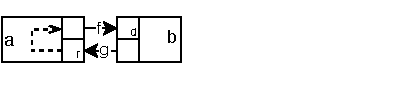
\includegraphics[width=0.5\textwidth]{images/simple_example.pdf}
  \caption{A simple co-simulation scenario ($S1$).}
  \label{fig:simpleexample}  
\end{wrapfigure}

The input variables involved in an algebraic loop in the scenario $S$ are:
\begin{align}
  \inputs{\algebraic{S}} \triangleq \algebraic{S} \cap \allinputs
\end{align}

A scenario is either simple or complex.
\begin{definition}\label{def:simpleScenario}
  A scenario $S$ is simple if $\mayReject = \emptyset \land \algebraic{S} = \emptyset$.
\end{definition}

A scenario is complex if it is not simple. Using \cref{def:simpleScenario} we conclude that the scenario ($S1$) in \cref{fig:simpleexample} is simple because $\algebraic{S1}=\emptyset$ and none of the SUs implement error estimation ($\mayReject_{S1}=\emptyset$). The scenario ($S2$) in \cref{fig:algebraic_example} is complex since $\algebraic{S2}=\{\inputvar{f}, \inputvar{g}, \outputvar{f}, \outputvar{g}\}$ meaning that all variables are a part of a cyclic dependency that should be solved using a fixed point.
The scenario ($S3$) in \cref{fig:step_finding_scenario} is also complex because SU $C$ implements error estimation ($\mayReject_{S2}=\{C\}$) and therefore can perform step rejection. Step rejection requires special attention since the orchestrator should backtrack the simulation and restart the simulation with a smaller step in case of a step rejection.

The reason for distinguishing between simple and complex scenarios is that the simulation strategy depends on the scenario type. This is treated in more detail later in the paper.
Next, we give a brief presentation of the contracts from \cite{Gomes2019a} before describing how they can be used to verify a co-simulation algorithm.

\begin{figure}[htb]
  \begin{subfigure}{0.48\textwidth}
    \centering
    \centering
    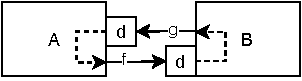
\includegraphics[width=0.9\textwidth]{images/scenario_algebraic.pdf}
    \caption{Scenario $S2$ with an algebraic loop.}
    \label{fig:algebraic_example}
  \end{subfigure}
  \begin{subfigure}{.48\textwidth}
    \centering
    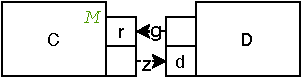
\includegraphics[width=0.95\textwidth]{images/step_negotiation_scenario.pdf}
    \caption{Scenario $S3$ needs step negotiation.}
    \label{fig:step_finding_scenario}
    \end{subfigure} 
    \caption{Complex co-simulation scenarios.}
    \vspace{-2em}

  \end{figure}

The contracts are described as preconditions of the SU-actions $\fget{}$, $\fset{}$ and $\fdoStep{}$.
It should be pointed out that each input and output has a timestamp referring to when it was last successfully activated by an action. 
%\vspace{-0.8em}
\begin{definition}[Get Action]\label{def:getout}  
  The precondition of $\fget{c}(\stateafter{c}{t}, \outputvar{c})$ is: \\
  $\forall (\inputvar{\dontcare}, \outputvar{c}) \in \feedthrough{c} \implies \inputvar{\dontcare} = \tuple{t_h, \dontcare} \land t_h = t$.\\
  Informally saying that all inputs that feeds through to $\outputvar{c}$ should be set.
  This criterion is denoted as the predicate: $\fpreget{c}: \stateset{c} \times \outputs{c} \to \mathbb{B}$.
\end{definition}
%\vspace{-1em}
\begin{definition}[Set Action]\label{def:setin}
  The precondition of $\fset{c}(\stateafter{c}{t}, \inputvar{c}, \inputV)$ depends on the contract of the input:
  \begin{compactitem}
    \item If $\inputvar{c} \in \allreactivity$ then the operation is valid if $\inputV= \tuple{t_h,\dontcare}, \textrm{ where } t_h = t+H$
    \item If $\inputvar{c} \in \alldelayed$ then the operation is valid if $\inputV= \tuple{t_h,\dontcare}, \textrm{ where } t_h = t$.
  \end{compactitem} 
  This informally says that the value set on $\inputvar{c}$ should be obtained at a meaningful point in time dictated by the input contract.
  We denote this as the predicate: $\fpreset{c}: \stateset{c} \times \inputs{c} \times \valuesExchanged  \to \mathbb{B}$.
  \end{definition}

  The criterion on a set-action will first have an effect when the SU is stepped. However, we found that it was easier to catch and correct an incorrect algorithm by moving this criterion to the set-action. 
  
  %\vspace{-1em}
  \begin{definition}[Step Computation]\label{def:step}
  The precondition of $\fdoStep{c}(\stateafter{c}{t}, H)$ is satisfied if all the following conditions are fulfilled:
  \begin{compactitem}
    \item $\forall \inputvar{c} \in \inputs{c} \ldotp \inputvar{c} \in \alldelayed \implies \inputvar{c} = \tuple{t_h,\dontcare} \land t_h = t$. 
    \item  $\forall \inputvar{c} \in \inputs{c} \ldotp \inputvar{c} \in \allreactivity \implies \inputvar{c} = \tuple{t_h,\dontcare} \land t_h = t + H$.
    %\item $\fdoStep{c}(\stateafter{c}{t},H)=(\dontcare,H)$
  \end{compactitem}
  Informally, this is that all inputs should set with a new value since the last time the SU was stepped.
  This is denoted as the predicate: $\fpredoStep{c}: \stateset{c} \times \stepbase \to \mathbb{B}$.
  \end{definition}
%\vspace*{-1.4em}
\begin{definition}[Preconditions of a Scenario]\label{def:precondition}
  The set of all preconditions $\precondition$ of a scenario is the union of the preconditions for each SU $c \in \fmus$:
  \begin{align}
    \precondition = \bigcup_{c \in \fmus} \set{\bigcup_{i \in \inputs{C}}\fpreset{c}(\dontcare, \inputvar{i}, \dontcare), \bigcup_{i \in \outputs{C}}\fpreget{c}(\dontcare, \outputvar{i}), \fpredoStep{c}}
  \end{align}
\end{definition}

The SU inspired by the FMI-standard~\cite{FMI2014} is a state-machine, the  SU as a state-machine.
The formalization in Maude enforces them, but they are treated in this paper.

\subsection{Co-simulation algorithms}\label{sc:cosimalgo}
A scenario is , as described, simulated by a co-simulation algorithm that consists of state-changing functions, an initialization procedure, and a co-simulation step. 
%This work concentrates on the co-simulation step, which we refer to as the algorithm throughout the paper. The other aspects of a co-simulation algorithm can trivially be derived from the method.  

The purpose of the co-simulation step is to advance all SUs $\fmus$, and all inputs and outputs $(\allinputs \cup \alloutputs)$, from the initial times $t$ to a future time $t+H, \textrm{ where } H > 0$. 
We use function $\ftime: \stateset{C} \to \timebase$ to obtain the current timestamp of an SU.
This makes it possible to define the Hoare-triple of the co-simulation step $P$:
\begin{align*}
  Hoare(P) \,\triangleq\, &\{\forall v \in \allinputs \cup \alloutputs \ldotp v = \tuple{t, \dontcare} \land \forall c \in \fmus \ldotp \ftime(\stateafter{c}{t}) = t\} \qquad  P \\
  & \qquad \{\forall v \in \allinputs \cup \alloutputs \ldotp v = \tuple{t+H, \dontcare} \land \forall c \in \fmus \ldotp \ftime(\stateafter{c}{t+H}) = t+H \}
\end{align*}

A co-simulation step $P$  is a sequence of instructions using the SU's functions $\fset{c},\fget{c}$, and $\fdoStep{c}$. 
Each index $i$ of the sequence $P[i]$ represents an action in the algorithm, for example, if $P$ is the co-simulation step in \cref{alg:algorithm_1} $P[0] = \fdoStep{A}(\stateafter{A}{0}, \dontcare)$. \Cref{fig:algorithms} shows three different co-simulation steps of the scenario in \cref{fig:simpleexample}. 
\vspace{-1em}
\begin{figure}[htb]
  \centering
  \begin{minipage}[t]{.325\textwidth}
    \begin{algorithm}[H]
      \caption{}
      \label{alg:algorithm_1}
      \begin{algorithmic}[1]
        \scriptsize
        \State $(\stateafter{A}{H},H) \gets \fdoStep{A}(\stateafter{A}{0}, H)$
        \State $(\stateafter{B}{H},H) \gets \fdoStep{B}(\stateafter{B}{0}, H)$
        \State $f_{v} \gets \fget{A}(\stateafter{A}{H}, \outputvar{f})$
        \State $g_{v} \gets \fget{B}(\stateafter{B}{H}, \outputvar{g})$
        \State $\stateafter{B}{H} \gets \fset{B}(\stateafter{B}{s}, \inputvar{f}, f_{v})$
        \State $\stateafter{A}{H} \gets \fset{A}(\stateafter{A}{H},\inputvar{g},g_{v})$
      \end{algorithmic}
    \end{algorithm}
  \end{minipage}
  \begin{minipage}[t]{0.325\textwidth}
    \begin{algorithm}[H]
      \caption{}
      \label{alg:algorithm_2}
      \begin{algorithmic}[1]
        \scriptsize
        \State $(\stateafter{B}{H},H) \gets \fdoStep{B}(\stateafter{B}{0}, H)$
        \State $(\stateafter{A}{H},H) \gets \fdoStep{A}(\stateafter{A}{0}, H)$
        \State $g_v \gets \fget{B}(\stateafter{B}{H}, \outputvar{g})$
        \State $\stateafter{A}{H} \gets \fset{A}(\stateafter{A}{H}, \inputvar{g}, g_v)$
        \State $f_v \gets \fget{A}(\stateafter{A}{H}, \outputvar{f})$
        \State $\stateafter{B}{H} \gets \fset{B}(\stateafter{B}{H}, \inputvar{f}, f_v)$
      \end{algorithmic}
    \end{algorithm}
  \end{minipage}
  \begin{minipage}[t]{0.325\textwidth}
    \begin{algorithm}[H]
      \caption{}
      \label{alg:algorithm_3}
      \begin{algorithmic}[1]
        \scriptsize
        \State $(\stateafter{B}{H},H) \gets \fdoStep{B}(\stateafter{B}{0}, H)$
        \State $g_v \gets \fget{B}(\stateafter{B}{H}, \outputvar{g})$
        \State $\stateafter{A}{0} \gets \fset{A}(\stateafter{A}{0}, \inputvar{g}, g_v)$
        \State $f_v \gets \fget{A}(\stateafter{A}{0}, \outputvar{f})$
        \State $\stateafter{B}{H} \gets \fset{B}(\stateafter{B}{H}, \inputvar{f}, f_v)$
        \State $(\stateafter{A}{H},H) \gets \fdoStep{A}(\stateafter{A}{0}, H)$
      \end{algorithmic}
    \end{algorithm}
    \vspace{4pt}
  \end{minipage}
  \vspace{-2em}
  \caption{Three algorithms conforming to the FMI Standard (version 2.0) of the scenario in \cref{fig:simpleexample}.}
  \label{fig:algorithms}
%  \vspace{-1em}
\end{figure}

Although the three algorithms in \cref{fig:algorithms} consist of the same actions, they are not equivalent, and simulating with one algorithm instead of one of the others could drastically change the co-simulation result as shown in \cite{Gomes2019c}. 
They showed that by obeying the contracts, the scenario will be simulated correctly. We assume that the contracts in the scenario are constant through the simulation, which is the case for most commercially used SUs.
At the end of \cref{sec:correctcosim}, we show which of these algorithms is correct.

A co-simulation step $P$ is executed using a configuration $c$. The configuration $c \triangleq \tuple{H, guess}$ consists of the parameters of the co-simulation step $P$.  $H \in \stepbase$ defines the step size, and $guess : \inputs{algebraic} \to \valuesExchanged$ is a total function linking all inputs in $\inputs{algebraic}$ to a guess that tries to satisfy the algebraic loops. Using the example from \cref{alg:algorithm_1}, the action at index 0 in $P$ applied with the configuration $\tuple{1,\dontcare}$ is: $P[0](c) = \fdoStep{A}(\stateafter{A}{0}, 1)$. The configuration defines the step size $(1)$ of the step-action. 

The set $\configuration$ denotes all the possible configurations of the co-simulation step for a given scenario. The execution of a co-simulation step $P$ is the execution of each action in $P$. We define such execution of $P$ using configuration $c$ as:
\vspace{-1em}
\begin{align}
  P(c) \triangleq \text{for each } i \in \dom{P} \ldotp P[i](c)
\end{align}
An execution of $P(c_j)$ yields another configuration $c_{j+1} \in \configuration$ where $P(c_j) = c_{j+1}$. The configuration $c_{j+1}: \tuple{H_1, guess_1}$ is obtained from the algorithm $P$ and configuration $c_j: \tuple{H, guess}$ by updating $H_1$ to the smallest step accepted by an SU during the execution of $P(c_j)$. And the function $guess_1$ has the same domain as $guess$, but the range is updated to the new value of the output coupled to the associated input in the domain of $guess$ after executing $P(c_j)$.
\vspace{-1em}
\begin{align}
  guess_{j+1}(u) = value(u,P(c_j)) \text{ and } H_1 = minStep(P(c_j))  
\end{align}  
The execution of a configuration $c: \tuple{H, guess}$ has converged if all SUs accept the step $H$, and all algebraic loops are stabilized (all values in the range of $guess$ are fixed-points). 
The domain of $guess$ is all the inputs in $\inputs{algebraic}$ for the scenario; this means that all configurations of the same scenario have the same domain.
\begin{definition}\label{def:convergent}
  Two configurations of the same scenario S $c_j:\tuple{H_1,guess_1} \in \configuration$ and $c_{j+1}: \tuple{H_2, guess_2} \in \configuration$ are convergent if:
  \vspace{-1em}
  \begin{align*}
    c_j \approx c_{j+1} \triangleq H_1 = H_2 \land (\forall i \in \dom{guess} \ldotp guess_1[i] \approx guess_2[i])
  \end{align*}
  Two values $v1_E: (v_1, t_1)$ and $v2_E: (v_2, t_2)$ of type $\valuesExchanged$ converge if:
  \begin{align}
    v1_E \approx v2_E \triangleq \, \mid v_1 - v_2 \mid \ \leq \epsilon \land t_1 = t_2
  \end{align}
\end{definition}

Formally an execution of a co-simulation step $P$ of a configuration $c_j$ is stable or has converged if $P(c_j) = c_{j+1} \implies c_j \approx c_{j+1}$.
% All configurations are stable for simple scenarios defined by \cref{def:simpleScenario}. 
% \begin{lemma}\label{def:simple}
%   A scenario is simple if all configurations of the algorithm $P$ converge: 
%   \begin{align*}
%     \forall c_j,c_{j+1} \in \configuration \ldotp P(c_{j}) = c_{j+1} \implies c_j \approx c_{j+1}
%   \end{align*}
% \end{lemma}

A complex scenario is a scenario where not all configurations are stable. Such a scenario can only be correctly simulated by an algorithm $P$ if a convergent configuration exists:
\vspace{-1em}
\begin{align}
  \exists c \in \configuration, \exists j \in \setnat \ldotp P(c_{j}) = c_{j+1} \implies c_{j} \approx c_{j+1}
\end{align}
Some measures should be taken to handle cases where no convergent configuration exists.

\subsection{Correct Co-simulation Algorithms}\label{sec:correctcosim}
To optimally simulate a co-simulation scenario using an algorithm $P$ requires more than a convergent configuration $c$. The algorithm $P$ should also successfully satisfy all the preconditions/contracts. To describe this, we introduce the sequence $\allcontracts$, which is a permutation of the set $\precondition$ (cf.\ \cref{def:precondition}).
The sequence $\allcontracts$ is constructed by a function $\allcontracts = \mathit{contracts(P, \precondition)}$ that for each action in $P$ finds the corresponding precondition $pre \in \precondition$ and adds it to $\allcontracts$ such that for an arbitrary index $i$ in $P$, $\allcontracts[i]$ is the precondition of the action $P[i]$.

If an action at index $i$ in $P$ satisfies its precondition $\allcontracts[i]$ using the configuration $c$, it is denoted as:
\vspace{-1em}
\begin{align}
  P[i](c) \models \allcontracts[i]
\end{align}
A co-simulation step $P$ using a configuration $c$ satisfies $\allcontracts$ if all actions satisfy its precondition. 
\vspace{-1em}
\begin{align}
  P(c) \models \allcontracts \triangleq \forall i \in \dom{P} \ldotp P[i](c) \models \allcontracts[i]
\end{align}
$P(c) \models \allcontracts$ means the algorithm respects the scenario's contracts.
Based on previous studies it is well-known that a non-convergent configuration $c$ does not respect all the contracts:
\vspace{-1em}
\begin{align}\label{eq:incorrectConf}
  c_j \not\approx c_{j+1} \implies P(c_j) \not\models \allcontracts
\end{align}
Therefore we only check the contracts of the scenario if the current configuration is convergent.
We can now describe what it means for an algorithm to be correct for a given scenario in the following Hoare triple.

\begin{definition}\label{def:correctalgo}
  An algorithm $P$ and configuration $c: \tuple{H, \dontcare}$ is correct if:
  \vspace{-0.5em}
  \begin{align*}
     P(c) \models \allcontracts \quad \land \quad
     &\{\forall v \in \allinputs \cup \alloutputs \ldotp v = \tuple{t, \dontcare} \land \forall c \in \fmus \ldotp \ftime(\stateafter{c}{t}) = t\} \quad P(c) \\
     & \{\forall v \in \allinputs \cup \alloutputs \ldotp v = \tuple{t+H, \dontcare} \land \forall c \in \fmus \ldotp \ftime(\stateafter{c}{t+H}) = t+H \}
  \end{align*}
  Meaning all preconditions are satisfied and all SUs and inputs have moved from time $t$ to time $t+H$ through the execution of $P(c)$.
\end{definition}
\vspace{-0.5em}

Using \cref{def:correctalgo} we conclude that \cref{alg:algorithm_3} is correct while the others are incorrect since they break one or more of the defined preconditions. \Cref{alg:algorithm_1,alg:algorithm_2} violate the precondition of $\fdoStep{b}$ on line 2 by stepping it without having provided SU $b$ with a value on the reactive input $f$. 
These definitions form the basis for describing the approach and implementation used to verify co-simulation algorithms in this work.


\section{Modeling Co-simulation Scenarios in Maude}
\label{sec:model}

This section describes how we model  individual SUs and their
composition in a co-simulation scenario in Maude.
%
Due to space limitations, we only provide fragments of our Maude
model. 
The entire model, including the synthesis and execution of co-simulation
algorithms (\cref{sc:synthesize}) and the synthesis of
instrumentations and parameters (\cref{sc:DSE})  is
available at \url{https://github.com/SimplisticCode/Co-simulation_WRLA} and consists of around 
1400 LOC. 

We formalize  co-simulation scenarios in an object-oriented style. The
 state is a term
 \texttt{\char123}$\mathit{SUs}\;\mathit{connections}\;\mathit{orchObjects}$\texttt{\char125}, 
 of sort \texttt{GlobalState}, 
 where $\mathit{SUs}$ is set of objects modeling simulation units,
$\mathit{connections}$ denote the port couplings, and
$\mathit{orchObjects}$ are two additional (orchestration) objects used
during synthesis and execution of co-simulation algorithms (see
\Cref{sc:synthesize}). 

We illustrate our  framework using a system where a
\emph{controller} 
controls the water level of a \emph{water tank} with constant inflow
of water,  by opening and closing a valve
at the bottom of the tank. 
The system can be modeled using  one SU for the tank and one for
the controller, and has the architecture shown in
\cref{fig:simpleexample}.

%\subsection{Simulation Units}
An simulation unit  is modeled as an object instance of the following
class: % a
                                % subsystem with parameters, ports, a
% state, and a time: 
\small
\begin{alltt}
class SU | time\,\,: Nat,                inputs\,\,: Configuration,
           outputs\,\,: Configuration,   canReject\,\,: Bool,
           fmistate\,\,: fmiState,       parameters\,\,: LocalState,
           localState\,\,: LocalState .
\end{alltt}
\normalsize

\noindent The attribute \texttt{time} denotes the time of the SU; 
\texttt{inputs} and \texttt{outputs} denote the objects modeling the
SU's input and output 
ports; \texttt{canReject}  is \texttt{true} if  the SU
implements error estimation (i.e., is an element of the set
$\mayReject$);  
\texttt{fmistate} denotes the \emph{simulation mode}
(see~\cite{FMI2014}) of the SU; \texttt{localState} denotes the SU's internal
state; and \texttt{parameters} denotes the values of the SU's
parameters. 

Input and output ports are modeled as  instances of the following
classes:

\small
\begin{alltt}
class Port | value\,:\,\,FMIValue, time\,:\,\,Nat, status\,:\,\,PortStatus, type\,:\,\,FMIType\,. 
class Input | contract : Contract .
class Output | dependsOn : OidSet .     
subclasses Input Output < Port .
\end{alltt}
\normalsize

\noindent The attributes \texttt{value} and \texttt{time} denote, respectively, the
value of the port and the time of its last set/get operation; 
\texttt{status} is \texttt{true}  if the port has been
updated  at the current time;   \texttt{contract} denotes the
input port's instrumentation/contract (\texttt{delayed} or
\texttt{reactive}); and 
\texttt{dependsOn} denotes the set of inputs that feed
through to the output port. 

\begin{example}
The initial state of the tank in our  example is modeled as an object
  
\scriptsize
\begin{alltt}
< "tank" : SU | parameters : ("flow" |-> <\,5\,>),  localState : ("waterlevel" |-> <\,0\,>),
                inputs : (< "valveState" : Input | value\,\,:\,\,<\,0\,>, time\,\,:\,\,0, contract\,\,:\,\,delayed >),
                outputs : (< "waterlevel" : Output | value : <\,0\,>, time : 0,
                                                     status : Undef, dependsOn : empty >)
                time : 0,  canReject : false >
\end{alltt}
\normalsize

\noindent The \texttt{tank} has one delayed input port and one output
port, and the local state indicates that the tank is empty.  
The parameter \texttt{flow} defines the amount of water that flows
into the tank per time unit.
\end{example}

To formalize the behaviors of an SU we formalize the functions
\texttt{set}, \texttt{get}, and \texttt{step} in
\cref{def:fmu}. 
For example, the $\fget{}$ operation that updates the \texttt{time}
and \texttt{status}  of a set
of output ports is formalized as follows:\footnote{We do not show
  variable declarations, but follow the convention that variables are
  written with capital letters.} 

\small
\begin{alltt}
  op getAction : Object OidSet -> Object .
  eq getAction(< SU1 : SU | >, empty) = < SU1 : SU | > .
  eq getAction(< SU1 : SU | time : T, 
                            outputs : (< O : Output | > OS) >, (O , P)) = 
     getAction(< SU1 : SU | outputs : 
                     (< O : Output | time : T, status : Def > OS) >, P) .
\end{alltt}
\normalsize

% The operator iterates over a defined set of output ports.
% The \textit{time} and \textit{state} of the output port is update to
% the time $T$ and the input is marked as defined \textit{Def}. 

%The precondition ($\fpreget{}$) is omitted from the operation
%\emph{getAction} since it is included in the functions calling it. 
%The functions $\fget{}$ and $\fset{}$ are similar for all SUs
%described in the framework. 

The concrete behavior of an SU is given by defining its $\fdoStep{}$
function:

\begin{example}
The following definition of the \texttt{step} function in our running
example says that  the water level of the tank changes according to
step \emph{duration} \texttt{STEP}, the parameter \texttt{flow}, and the
state (\texttt{value}) of the input \texttt{valve}:

\scriptsize
\begin{alltt}
eq step(< "tank" : SU | time : T, parameters : ("flow" |-> <\,FLOW\,>), 
                        inputs : < "valve" : Input | value : <\,STATE\,> >, 
                        outputs : < "waterlevel" : Output | time : T >,
                        localState : ("waterlevel" |-> <\,LEVEL\,>) >,
        STEP) = 
  if STATE == 1 then    \emph{--- valve is open}
    < "tank" : SU | time : (T\,+\,STEP), localState : ("waterlevel" |-> <\,0\,>),
          outputs : < "waterlevel" : Output | value\,\,:\,\,<\,0\,>, time\,\,:\,\,(T\,+\,STEP), status\,\,:\,\,Undef > >
  else                  \emph{--- valve is closed}
    < "tank" : SU | time : (T\,+\,STEP),  localState : ("waterlevel" |-> <\,LEVEL\,+\,(STEP\,*\,FLOW)\,>), 
                    outputs : < "waterlevel" : Output | value : < LEVEL + (STEP * FLOW) >, 
                                                        time : (T + STEP), status : Undef > > 
  fi .
\end{alltt}
\normalsize
\end{example}

%A scenario is a collection of SUs composed using a set of couplings/connections.
A connection/coupling connecting the output port $o$ of SU $\mathit{su}_1$ to
the input port $i$ of SU $\mathit{su}_2$ is represented by the term
\texttt{"}$\mathit{su}_1$\texttt{"} \texttt{!} \texttt{"}$o$\texttt{"} \texttt{==>}
\texttt{"}$\mathit{su}_2$\texttt{"} \texttt{!} \texttt{"}$i$\texttt{"} of a subsort
\texttt{Connection} of sort \texttt{Configuration}.


% ports connects an output with an input:
% \begin{alltt}
%   \small
% op _==>_ : EPortId EPortId -> Connection [ctor] .
% subsort Connection < Configuration .
% \end{alltt}

We define scenarios by defining constants \texttt{simulationUnits}
and \texttt{externalConnection} that denote, resp.,  the
simulation unit objects and  their connections. 

\begin{example}\label{ex:simulationunits}
The SUs and the couplings in our  example are defined as
follows:

\scriptsize
\begin{alltt}
eq simulationUnits = 
   < "tank" : SU | parameters : ("flow" |-> <\,100\,>),  localState : ("waterlevel" |-> <\,0\,>),
                   time : 0,  fmistate : Instantiated, canReject : false, 
                   inputs : (< "valveState" : Input | value : <\,0\,>, type : integer, time : 0,
                                                      contract : delayed, status : Undef >), 
                   outputs : (< "waterlevel" : Output | value : <\,0\,>, type : integer, time : 0,
                                                        status : Undef, dependsOn : empty >) >

   < "ctrl" : SU | parameters : (("high" |-> <\,5\,>) , ("low" |-> <\,0\,>)), canReject : false, 
                   localState : ("valve" |-> <\,false\,>), fmistate : Instantiated, time : 0, 
                   inputs : (< "waterlevel" : Input | value : <\,0\,>, type : integer, time : 0,
                                                      contract : reactive, status : Undef >), 
                   outputs : (< "valveState" : Output | value : <\,0\,>, type : integer, time : 0,
                                                        status : Undef, dependsOn : empty >) > .

eq externalConnection = ("tank" ! "waterlevel" ==> "ctrl" ! "waterlevel") 
                        ("ctrl" ! "valveState" ==> "tank" ! "valveState") .
\end{alltt}
\normalsize
\end{example}

%A scenario is described as a multiset of SUs and connections linking the ports.
%A simulation is instantiated as a \textit{GlobalState} using the equation:
The constant \texttt{setup} defines the initial state, and adds
appropriate initialized orchestration objects to the scenario:

\small
\begin{alltt}
op setup : -> GlobalState .
ceq setup = \char123INIT\char125
  if SCENARIO := externalConnection simulationUnits
  /\char92 validScenario(SCENARIO)
  /\char92 LOOPS := tarjan(SCENARIO)
  /\char92 NeSUIDs := getSUIDsOfScenario(SCENARIO)
  /\char92 INIT := calculateSNSet(SCENARIO OData(1,LOOPS, NeSUIDs)) .
\end{alltt}
\normalsize

\noindent The function \texttt{validScenario} checks whether all inputs are coupled and that no input has two sources.   
The function \texttt{tarjan} returns (a possibly empty) set  of algebraic loops in the scenario by searching for non-trivial strongly connected components in
the graph constructed using the rules  in \cite{Gomes2019c}.   
The function \texttt{getSUIDsOfScenario} returns  the set of all SU
identifiers. Finally, \texttt{calculateSNSet} checks if step negotiation 
should be applied in the simulation of the scenario, and generates a
global initial state with orchestration objects that store information
about the discovered algebraic loops and whether step negotiation is
needed.

\section{Model checking Analysis of co-simulation}
The non-deterministic rewrites rule in Maude allows exploration multiple instrumentations, 


\subsection{Orchestration Algorithms}
\begin{lemma}
\end{lemma}
All constructed orchestration algorithms of an instrumented scenario produce a deterministic co-simulation result.

This is verified using the following search:
\begin{lstlisting}
search (runAnyAlgorithm SCENARIO)  =>! S:SimulationState .
\end{lstlisting}

The search command relies heavily on rewriting rules generating the different orchestration algorithms for the instrumented scenario which afterwards will be .  

\subsection{Design Space Exploration}
Design Space Exploration is the 

\subsubsection{Instrumentation of Scenario}
The beginning adaption of contracts for input ports to achieve more accurate co-simulation results. 
A prominent problem in this domain is that most tools used for generating SUs (FMUs) do not export this information.


Find instrumentations leading to a desired co-simulation result - simple example. 



Furthermore, it is possible to restrict the explored instrumentations to a set satisfying specific properties such as no algebraic loops.
This restriction is, in fact, desirable in many applications where the orchestration engine does support these and also for simulations of real-time systems.

\subsubsection{Parameters of the Simulation Units}
A simulation unit has 



We can potentially use SMT-solving later to help us with the design space exploration.


We have performed the analyses on different scenarios. 
The state-space explosion is, of course, also applying to our work. 
However, we have been able to find the correct instrumentation and the contracts on systems with XX SUs.

Our test examples include the industrial case study original from Boeing presented in (Add reference to Gomes). 


\section{Synthesize of instrumentations and Parameters}\label{sc:DSE}
Using Maude's integrated LTL model checker, the Maude framework enables different kinds of design space exploration.
Design space exploration allows the co-simulation practitioner to explore how different model parameters/designs change the behavior of the system/simulation result.
The framework enables a co-simulation practitioner to experiment with different valuations of the scenario's instrumentation and model parameters.
We describe the two independently even though they can be combined.


\subsection{Instrumentation of a Scenario}
The instrumentation of the input ports is used to achieve more accurate co-simulation results as shown in \cite{Gomes2019,Oakes2021,hansen_verification_2021}.
However, finding the instrumentation that results in the most accurate simulation can be challenging since none of the existing tools to export FMUs/SUs provide this information.

To ease the transition, we use Maude's model checker to explore the consequences of using different instrumentations of a scenario.

To explore different instrumentations of a scenario, we define the contract: \emph{noContract}.
The contract can be used if the user does not know the input's contract.
A scenario where at least one of the input's contracts are annotated with \emph{noContract} is called \emph{uninstrumented}.
A scenario is \emph{instrumented} if no input in the scenario has a contract defined to be \emph{noContract}.

A scenario can only be simulated if it is instrumented since the rewrite rules only cover inputs with \emph{delayed} or \emph{reactive} contracts.

This allows Maude to play with different instrumentations of the scenario such that for each input with the contract \textit{noContract} Maude tries to perform a simulation where the input is delayed and a simulation where the input is reactive.
The rewriting rules for this is given below:
\begin{alltt}
  \small
rl [instr-delayed]: 
findInstr(< SU1 : SU | inputs : (< I : Input | contract : noContract > IS) > C)
=>
findInstr(< SU1 : SU | inputs : (< I : Input | contract : delayed > IS) > C) .

rl [instr-reactive]: 
findInstr(< SU1 : SU | inputs : (< I : Input | contract : noContract > IS) > C)
=>
findInstr(< SU1 : SU | inputs : (< I : Input | contract : reactive > IS) > C) .

crl [remove-findInstr]: findInstr(CONF) => CONF 
  if allConstraintsDefined(CONF) .
\end{alltt}

The co-simulation practitioner can use the rewriting rule below to experiment with different instrumentations of the scenario.

\begin{alltt}
  \small
  crl [findInstrumentation]: findContacts(INIT) => CONF
      if findInstr(INIT) => CONF
      \(\land\) empty == tarjan(CONF) *** No loops
      \(\land\) runAnyAlgorithm CONF => run: ORC on: FINAL with: SIMDATA
      \(\land\) shouldSatisfy(FINAL) .
  \end{alltt}

The rule generates all the different instrumentations of the scenario that satisfy specific properties.
It does so by first instrumenting the scenario to generate the instrumented scenario ``CONF''.
Hereafter it simulates the instrumented scenario ``CONF'' to check the resulting simulation.
The user can limit the explored instrumentations in desired ways by defining specific properties of the instrumentation.
For example, in the rule above, it is specified that none of the instrumentations must generate a complex scenario with algebraic loops.

The co-simulation practitioner can also specify concrete constraints on the simulation result.
The constraints are above specified using the predicate \emph{shouldSatisfy}.

The different instrumentations are explored using Maude's search command.

\begin{alltt}
  \small
  search findContacts(Scenario) =>! C:Configuration .
\end{alltt}
  
This returns all the configurations/instrumentations of the scenarios that satisfy the desired properties defined in the above rule.

\subsubsection{Parameters of the Simulation Units}
An SU may have different parameters affecting its behavior; an example is the desired temperature of an incubator.
This means that different parameters potentially lead to different simulation results.
Design space exploration explores how different valuations of the parameters affect the co-simulation result to find the optimal design of the system. 

The Maude framework allows design space exploration by letting the user specify the valuation a parameter as a set of possible valuations inside the \emph{choose}-operator as we shown below.
\begin{alltt}
  \small
< "tank" : SU | parameters : ("flow" |-> choose((< 1 >,< 2 >,< 30 >))) >
\end{alltt}

The \emph{choose}-operator non-deterministically picks an element of the defined set.
Using the \emph{choose}-operator and the model checker enables one to explore all the combinations of different valuations for the parameters.
The combinations are explored using the following rewriting rule:

\begin{alltt}
  \small
  crl [dse] : selectParams(UNITIALIZEDCONF) => CONF 
  if UNITIALIZEDCONF => CONF
  \(\land\) runAnyAlgorithm CONF => 
      run: < ALG : AlgData | Initialization : emptyList, 
      CosimStep : emptyList, Termination : emptyList > 
      on: FINALSTATE
      with: SIMULATIONDATA
  \(\land\) above10(FINALSTATE) .
\end{alltt}

The rule selects a parameter valuation and uses the valuation to perform a simulation.
After a simulation, we evaluate the design by checking the simulation's final state to ensure it satisfies specific user-defined properties.
In the above rule, the valuation must ensure that the simulation satisfies the predicate \emph{above10}.

The search of the design space exploration is in Maude performed using the search command starting from a scenario with multiple valuations.
\begin{alltt}
  \small
  search selectParams(ScenarioDSE)  =>! C:Configuration .
\end{alltt}

\subsubsection{Combining Design Space Exploration of the Instrumentation and Parameters}
The two searches described above can be combined. A co-simulation practitioner can simultaneously experiment with the instrumentation and the parameters to obtain the most accurate simulation while searching for the optimal system design.

This is concretely done by defining an uninstrumented scenario with changeable parameters.
% \subsection{Limitation of the approach}
% We have performed the analyses on different scenarios. 
% The state-space explosion is, of course, also applying to our work. 
% However, we have been able to find the correct instrumentation and the contracts on systems with \simon{Create big scenario and test} SUs.

% Also, we do not currently support adaptive co-simulations~\cite{Inci2021} where the instrumentation changes during the simulation. 
% However, this is our impression that this feature trivial can be added.

\section{Related Work}\label{sc:related}

\paragraph{Contracts - Gomes}
We do the instrumentation of 

\paragraph{Verification of co-simulation algorithms}
We look at real systems + Verification of behaviour properties - do take the real system 

Design Space Exploration

\paragraph{Synthesizing of co-simulation algorithms}



The study of semantics and verification of co-simulation algorithms is presented in \cite{Gomes2019c,Gomes2019a,Broman2013}. 
The paper \cite{Gomes2019c} describes a formalization of an FMI-based co-simulation scenario where several correctness criteria are placed on the co-simulation algorithm to generate and verify a co-simulation algorithm. 
This paper extends their work by treating co-simulation scenarios subject to algebraic loops and adaptive steps.
Thule et al. \cite{Thule_2018} studied how a co-simulation scenario's characteristics can be used to choose the correct simulation strategy for a given co-simulation algorithm. 
In \cite{thrane2021}, algorithms of complex scenarios are described, but this paper lacks the feature to verify the correctness of algorithms for complex scenarios.

Broman et al. describe in \cite{Broman2013} an approach to achieve deterministic co-simulation results by placing constraints on the co-simulation scenario to avoid algebraic loops. 
They also propose a generic master algorithm for handling step negotiation. 
However, such generic algorithms do not consider other constraints on the SUs like reactive inputs or algebraic loops. This paper deals with all these constraints.

Formal methods have previously been successfully used in the area of co-simulation \cite{Amalio2016,sampaio_behavioural_2016,cerone_formalising_2018}.
Amálio et al.\ \cite{Amalio2016} study how connections between simulation units can be formalized. They investigate how different formal tools can detect algebraic loops to obtain a deterministic co-simulation result. 
Cavalcanti et al.\ \cite{sampaio_behavioural_2016} claim to provide the first behavioral semantics of FMI. The paper shows how to prove essential properties of master algorithms, like termination and determinism. It also shows that the example provided in the FMI standard is not a valid algorithm. The paper \cite{cerone_formalising_2018} by Zeyda et al. formalizes models and proofs about co-simulation in Isabelle/UTP, illustrated by an industrial case study from the railway sector. 
However, their approach does not cover complex scenarios, unlike ours.

Nyman et al. in \cite{jensen_integrating_2017} examine how UPPAAL can analyze controller-based systems with FMUs and a master algorithm modeled in UPPAAL. UPPAAL was used to verify the properties of the controller used in the co-simulation. Palmieri et al. in \cite{palmieri2019framework} have used UPPAAL to provide sound guarantees on the interleaving between a graphical user interface and a generic FMI master algorithm. 
Our approach is more generic and relies on a parameterized template approach applied to arbitrary co-simulation scenarios subject to step negotiation and algebraic loops.

\simon{Add references to synthesizing papers, verification paper}

\section{Concluding Remarks}\label{sc:summary}
This work proposed how rewriting logic can be used to formalize co-simulation semantics such that correct-by-construction co-simulation algorithms can be synthesized and executed.
The approach can handle complex co-simulation scenarios subject to algebraic loops and step rejections.

We demonstrated using model checking that all implementation-aware algorithms of a scenario result in the same co-simulation result.
Furthermore, we presented how a co-simulation practitioner can integrate Maude into the development cycle to explore different system designs and find the optimal parameters and instrumentation of the system.

A future research agenda could into how the formalization could be connected with orchestration engines such that the synthesized algorithms could be executed on real-world simulation units described by the FMI standard.
The parameter search can potentially be explored symbolic.

Future work also includes formalizing the FMI 3.0 standard, which is still under development.
We will use our experience from this work to interact with the FMI steering committee and show them how different semantics affect the simulation result.

\paragraph{Acknowledgements}
We will like to thank Claudio Gomes, Peter Gorm Larsen, Jaco van de Pol, Stefan Hallerstede, and Jose Meseguer for their support and feedback on the work.
%
% ---- Bibliography ---


\bibliographystyle{splncs04}
\bibliography{bib}

\end{document}
